\section{Overview}
%URN构主要由vRNIC(前端和后端)和URN core两大部分组成。vRNIC是一个半虚拟化的RDMA网卡设备,每个vRNIC都有一对前后端,通过前后端的交互为guest提供虚拟的RDMA服务;URN 是对vRNIC虚拟RDMA的管理模块。此外, 对host和容器的verbs进行了修改以以便与URN框架协作。
The architecture of URN is shown in Figure~\ref{fig:framework-overview}. URN mainly consists of the vRNIC (virtual RDMA Network Interface Controller) and the URN core. The vRNIC is a para-virtualized virtual device for the guest environment, which includes a pair of frontend and backend modules; the URN core is a management unit for all vRNIC instances on the host. Besides, some modifications are required for  verbs libraries on the host and inside the containers to interact with the URN.

\begin{figure}[!ht]
	\centering
	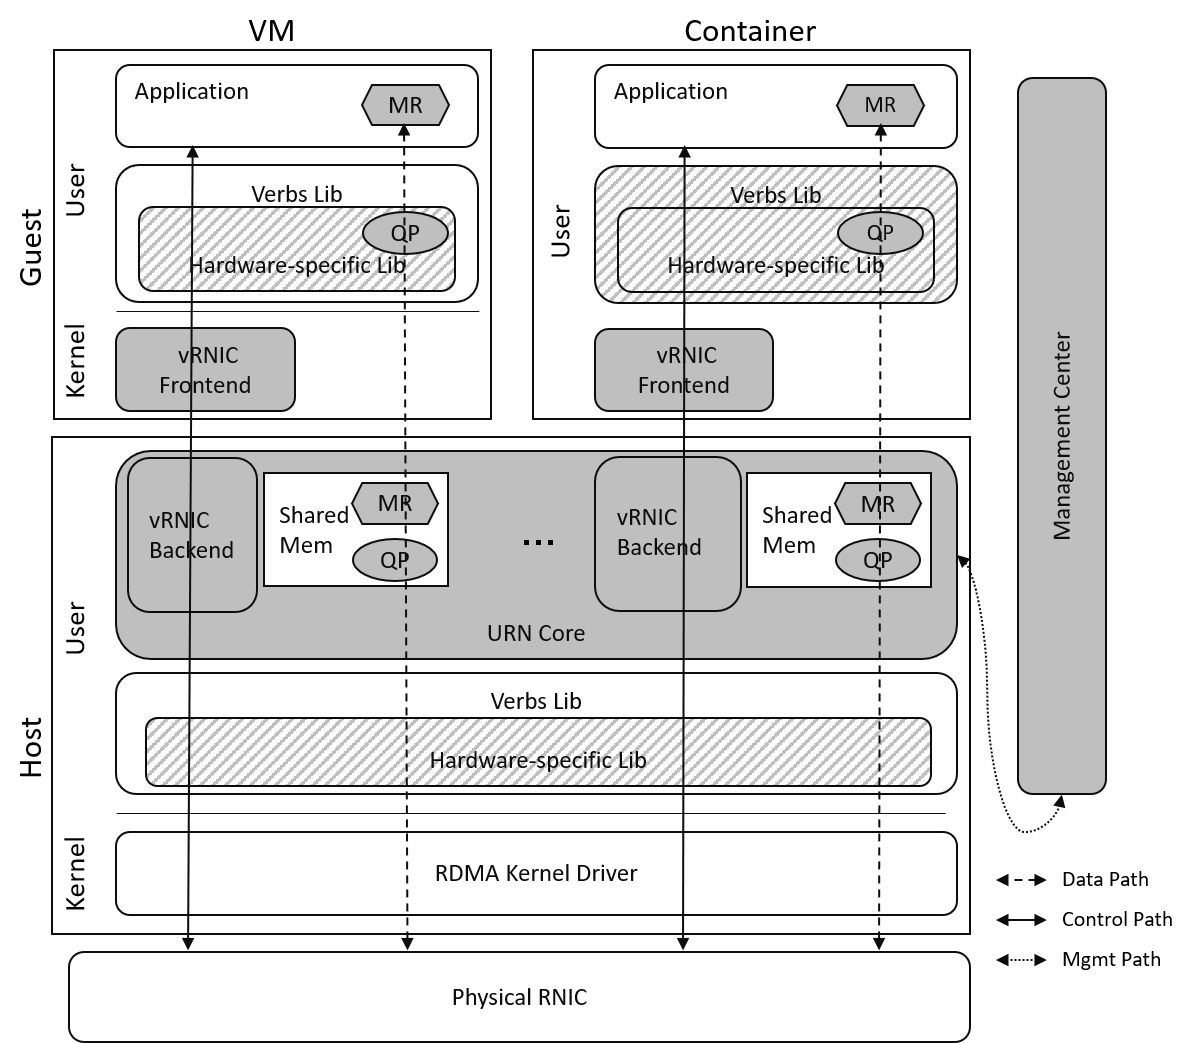
\includegraphics[width=1\linewidth]{images/framework-overview.png}
	\caption{Architecture Overview: The URN core manages all RDMA control path and data path can directly access physical RNIC through shared memory}
	\label{fig:framework-overview}
\end{figure}

% (1) vRNIC Frontend(FE): FE位于guest,是一个虚拟的RDMA网卡接口提供给上层verbs。Guest应用可以通过verbs库直接使用FE。在虚拟机里,FE在guest内核,通过与原RDMA内核驱动一致的接口与verbs库交互;在容器里,FE是一个用户库,容器应用使用修改的verbs库时链接FE,并通过定制化的接口与FE交互,该过程无需再陷入到主机内核。
(1) vRNIC Frontend: locates in the guest environment acting as the interface of the vRNIC. Applications in the guest environment can use the vRNIC interface through Verbs library. For VMs, the frontend virtual device is in guest kernel space and is designed to expose interfaces the same way as the RDMA device driver to the upper unmodified Verbs library. For containers, the frontend module is provided as a library that is linked to the applications aloneside with Verbs library.

% (2) vRNIC Backend(BE): BE位于host的用户空间,是vRNIC的虚拟设备后端。BE虚拟化了所有的RDMA网卡属性,例如QP。BE通过URN Core进行实例化,并通过修改过的Verbs库与RDMA物理网卡交互,维持RDMA上下文并提供给FE。在RDMA控制路径,BE和通常半虚拟化一致,执行FE转发的操作并返回给FE。在数据路径,应用直接在guest用户空间使用已经与BE映射的RDMA资源。
(2) vRNIC Backend: locates in the host user space. vRNIC backend is virtual device, which maintains three sets of information: a) attributes and contexts known by the physical RDMA device, e.g. QP, MR; b) attributes and contexts known by the virtual RDMA device in the guest environment; c) the mappings between virtual and physical attributes and contexts. vRNIC Backends are instantiated by the URN core. They interact with physical RNIC through unmodified Verbs libraries in the host environment. vRNIC Backend acts like an RDMA application in the host environment and delegates all the requests from vRNIC Frontend in the control path. In the data path, the key RDMA resources of the user applications in the guest environment, e.g. QPs and MRs, are directly mapped to the physical RDMA device. Both vRNIC Frontend and Backend are bypassed in the data path.

%(3)URN core:每台主机都有一个URNC core位于用户空间, 负责管理本地的RDMA虚拟网络,包括实例化BE、映射虚拟RDMA连接和配置路由等。URN core与修改过的Verbs用户库交互,再通过原生RDMA内核驱动实现对RDMA网卡的控制。
(3) URN core: There is one URN core instance in each host's user space. URN core is designed to manage the virtual and physical RDMA resources for the host, including instantiating vRNIC backends, managing virtual RDMA network configurations and policies. URN core also interact with physical RNIC through Verbs libraries. 

% (4) 管理中心: 整个集群有一个管理中心
(4) Management Center: There is one management center in the cluster. With the help of management center, control policies can be defined and influence each guest, e.g. QoS, ACL. More details will be discussed in section xxx.

% 此外,本文对容器的verbs库和主机verbs库进行了少量修改。在容器的修改,让Verbs库可以直接在用户空间与FE交互, 不用经过主机内核。在主机的修改,以支持RDMA后端使用共享内存对QP和MR等资源进行映射。为了实现与应用程序的透明性,上述修改均未破坏RDMA应用与Verbs库的API。
In addition,  we modified the Verbs libraries in containers so that the RDMA Verbs requests made to the kernel drivers can be redirected to the vRNIC Frontends. Note that Verbs APIs in the guest environment are not modified so that URN transparent to the guest RDMA applications. A few APIs in the Verbs library in the host user space are modified to support specifying a given memory address to be registered to the physical RNIC devices as key resource memory such as QP and MR. Currently, vanilla Verbs APIs don't allow applications to specify the address of resource memory region. But this capability is essential for URN to establish a zero-copy data path in the virtual environment. This will be discussed in detail in section XX.
